\subsection{Liftings}

Let \(r \in \mathbf{N}_{\mathbb{K}}\) and let \(g: \mathbf{X} \to \mathbf{Y}\) be a morphism of manifolds of class \(\mathbf{C}^{r+1}\) .

8.6.1. A lifting of g in T(Y) is a map \(\psi: X \to T(Y)\) such that the diagram

\pandocbounded{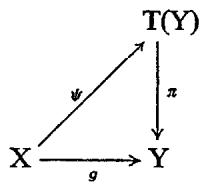
\includegraphics[keepaspectratio]{images/part001_bb2423ff.jpg}}

is commutative, \(\pi\) denoting the canonical projection of T(Y) onto Y. The data of \(\psi\) is equivalent to that of a section of the vector bundle \(g^{*}\mathrm{T}(\mathrm{Y})\), the inverse image under g of T(Y).

The notion of lifting generalizes that of a vector field (to which it reduces when \(g = \operatorname{Id}_{\mathbf{X}}\) ); an important part of the definitions and results concerning \(\theta_{\xi}\) and \(i(\xi)\) extends to liftings; we shall limit ourselves to briefly indicating a few of them.

8.6.2. Let \(\psi: X \to T(Y)\) be a lifting of \(g: X \to Y\) , and let \(\omega\) be a differential form of degree \(p\) on \(Y\) , with values in a vector bundle \(F\) with base \(Y\) . When \(p \geqslant 1\) , one denotes by \(i(\psi,\omega)\) or \(i(\psi)\omega\) or \(i_{\psi}(\omega)\) the differential form on X, of degree \(p-1\) , with values in \(g^{*}\mathbf{F}\) , such that

\[
i (\psi , \omega) _ {x} (v _ {1}, \dots , v _ {p - 1}) = \omega_ {g (x)} (\psi (x), T _ {x} (g). v _ {1}, \dots , T _ {x} (g). v _ {p - 1})\tag{1}
\]

for all \(x \in X\) and every family \(v_1, \ldots, v_{p-1}\) of elements of \(\mathbf{T}_x(X)\) . When \(p = 0\) , we set \(i(\psi, \omega) = 0\) . We say that \(i(\psi, \omega)\) is the interior product of \(\psi\) and of \(\omega\) ; if \(\psi\) and \(\omega\) are of class \(\mathbf{C}^r\) , then so is \(i(\psi, \omega)\) . Let \(\mathbf{F}' \times_{\mathbb{Y}} \mathbf{F}'' \to \mathbf{F}\) be a pairing of vector bundles with base Y. For \(\omega' \in {}^\tau \Omega^{p'}(Y; F')\) and \(\omega'' \in {}^\tau \Omega^{p''}(Y; F'')\) , one has

\[
i (\psi) \left(\omega^ {\prime} \wedge \omega^ {\prime \prime}\right) = (i (\psi) \omega^ {\prime}) \wedge g ^ {*} \omega^ {\prime \prime} + (- 1) ^ {p ^ {\prime}} g ^ {*} \omega^ {\prime} \wedge i (\psi) \omega^ {\prime \prime}.\tag{2}
\]

8.6.3. Examples

\begin{enumerate}
\def\labelenumi{\alph{enumi})}
\tightlist
\item
  A vector field \(\xi\) on X defines a lifting T(g) \(\circ\) \(\xi\) of g in T(Y), and we have:
\end{enumerate}

\[
i (\mathrm{T} (g) \circ \xi) = i (\xi) \circ g ^ {*}.\tag{3}
\]

\begin{enumerate}
\def\labelenumi{\alph{enumi})}
\setcounter{enumi}{1}
\tightlist
\item
  A vector field \(\eta\) on Y defines a lifting \(\eta \circ g\) of \(g\) in T(Y), and we have:
\end{enumerate}

\[
i (\eta \circ g) = g ^ {*} \circ i (\eta).\tag{4}
\]

\begin{enumerate}
\def\labelenumi{\alph{enumi})}
\setcounter{enumi}{2}
\tightlist
\item
  More generally, let \(h: \mathbf{Y} \to \mathbf{Z}\) be a morphism of manifolds of class \(\mathbf{C}^{r+1}\) . If \(\psi\) is a lifting of \(g\) to \(\mathbf{T}(\mathbf{Y})\) , then \(\mathbf{T}(h) \circ \psi\) is a lifting of \(h \circ g\) to \(\mathbf{T}(\mathbf{Z})\) and we have:
\end{enumerate}

\[
i (\mathrm{T} (h) \circ \psi) = i (\psi) \circ h ^ {*}.\tag{5}
\]

If \(\varphi\) is a lifting of \(h\) to \(\mathrm{T}(Z)\) , then \(\varphi \circ g\) is a lifting of \(h \circ g\) to \(\mathrm{T}(Z)\) and we have:

\[
i (\varphi \circ g) = g ^ {*} \circ i (\varphi).\tag{6}
\]

8.6.4 (“Infinitesimal transformations”). Let \(\psi\) be a lifting of class \(C^r\) of \(g\) and let \(\omega\) be a differential form of degree \(p\) on Y, taking values in a Banach space F, and of class \(C^r\) . The differential form on X

\[
d (i (\psi) \omega) + i (\psi) d \omega\tag{7}
\]

is of degree \(p\) and of class \(\mathbf{C}^{r-1}\) ; it is denoted \(\theta_{\psi}.\omega\) .

If f is a function of class \(C^{r}\) on X, we have

\[
\theta_ {f \psi}. \omega = d f \wedge i (\psi) \omega + f \theta_ {\psi}. \omega .\tag{8}
\]

8.6.5 ("Characterization of \(\theta_{\psi}.\omega\) as derivative"). Keep the hypotheses of 8.6.4. Let \(x\in X\) . There then exists an open neighborhood U of \(x\) , an open neighborhood I of 0 in K, and a morphism G: I × U → Y of class \(C^{r}\) having the following two properties:

\begin{enumerate}
\def\labelenumi{\alph{enumi})}
\item
  For every \(x \in \mathbf{U}\) , one has \(\mathbf{G}(0, x) = g(x)\) .
\item
  For every \(x \in \mathbf{U}\) , the image under \(\mathrm{T}_{(0,x)}(\mathrm{G})\) of the tangent vector (1, 0) is equal to \(\psi(x)\) .
\end{enumerate}

Suppose that (U, I, G) satisfies these conditions; for every \(t \in \mathbf{I}\) , denote by \(\mathbf{G}_t\) the map \(x \mapsto \mathbf{G}(t, x)\) from U to Y; set \(\omega_t = \mathbf{G}_t^*(\omega)\) . For every \(x \in \mathbf{X}\) , the map \(t \mapsto \omega_t(x)\) from I to \(\operatorname{Alt}^p(\mathrm{T}_x(\mathbf{X}), \mathbf{F})\) is of class \(\mathbf{C}^r\) , and its derivative at the origin is given by the formula

\[
\frac {d}{d t} (\omega_ {t} (x)) _ {t = 0} = (\theta_ {\psi}. \omega) (x).\tag{9}
\]

